\documentclass[tikz,border=3pt]{standalone}
\usepackage[utf8]{inputenc}
\usepackage[T1]{fontenc}
\usepackage{lmodern}
\renewcommand{\familydefault}{\sfdefault}
\usepackage{sansmath}\sansmath
\usepackage{chemfig}
\usepackage{pgfplots}\pgfplotsset{compat=1.18,/pgf/number format/use comma,/pgf/number format/1000 sep={.}}
\usetikzlibrary{arrows.meta,calc,positioning,decorations.pathmorphing,patterns}
% paleta del sitio
\definecolor{nar}{HTML}{E8680C}\definecolor{narc}{HTML}{FFB35C}\definecolor{hielo}{HTML}{FFF3E8}
\definecolor{tinta}{HTML}{1D1D1F}\definecolor{gris}{HTML}{6E6E73}\definecolor{lila}{HTML}{7C5CF0}
\definecolor{azul}{HTML}{2F6FD6}\definecolor{menta}{HTML}{17A673}\definecolor{coral}{HTML}{E8342A}
\begin{document}
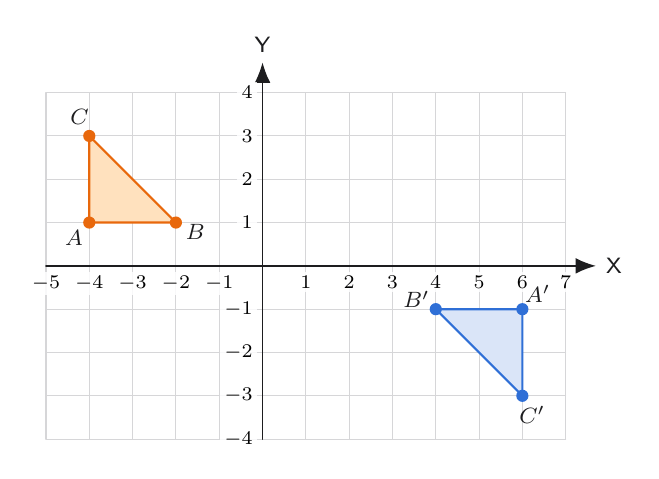
\begin{tikzpicture}[font=\small,x=0.55cm,y=0.55cm,line cap=round,line join=round,step={(1,1)}]
\draw[gris!28,thin] (-5,-4) grid (7,4);
\draw[-{Latex[length=2.6mm,width=2mm]},tinta,semithick] (-5,0)--(7.7,0) node[right,font=\footnotesize] {X};
\draw[-{Latex[length=2.6mm,width=2mm]},tinta,semithick] (0,-4)--(0,4.7) node[above,font=\footnotesize] {Y};
\node[below,font=\scriptsize,inner sep=1.5pt,fill=white,fill opacity=.85,text opacity=1] at (-5,-0.12) {$-5$};
\node[below,font=\scriptsize,inner sep=1.5pt,fill=white,fill opacity=.85,text opacity=1] at (-4,-0.12) {$-4$};
\node[below,font=\scriptsize,inner sep=1.5pt,fill=white,fill opacity=.85,text opacity=1] at (-3,-0.12) {$-3$};
\node[below,font=\scriptsize,inner sep=1.5pt,fill=white,fill opacity=.85,text opacity=1] at (-2,-0.12) {$-2$};
\node[below,font=\scriptsize,inner sep=1.5pt,fill=white,fill opacity=.85,text opacity=1] at (-1,-0.12) {$-1$};
\node[below,font=\scriptsize,inner sep=1.5pt,fill=white,fill opacity=.85,text opacity=1] at (1,-0.12) {$1$};
\node[below,font=\scriptsize,inner sep=1.5pt,fill=white,fill opacity=.85,text opacity=1] at (2,-0.12) {$2$};
\node[below,font=\scriptsize,inner sep=1.5pt,fill=white,fill opacity=.85,text opacity=1] at (3,-0.12) {$3$};
\node[below,font=\scriptsize,inner sep=1.5pt,fill=white,fill opacity=.85,text opacity=1] at (4,-0.12) {$4$};
\node[below,font=\scriptsize,inner sep=1.5pt,fill=white,fill opacity=.85,text opacity=1] at (5,-0.12) {$5$};
\node[below,font=\scriptsize,inner sep=1.5pt,fill=white,fill opacity=.85,text opacity=1] at (6,-0.12) {$6$};
\node[below,font=\scriptsize,inner sep=1.5pt,fill=white,fill opacity=.85,text opacity=1] at (7,-0.12) {$7$};
\node[left,font=\scriptsize,inner sep=1.5pt,fill=white,fill opacity=.85,text opacity=1] at (-0.12,-4) {$-4$};
\node[left,font=\scriptsize,inner sep=1.5pt,fill=white,fill opacity=.85,text opacity=1] at (-0.12,-3) {$-3$};
\node[left,font=\scriptsize,inner sep=1.5pt,fill=white,fill opacity=.85,text opacity=1] at (-0.12,-2) {$-2$};
\node[left,font=\scriptsize,inner sep=1.5pt,fill=white,fill opacity=.85,text opacity=1] at (-0.12,-1) {$-1$};
\node[left,font=\scriptsize,inner sep=1.5pt,fill=white,fill opacity=.85,text opacity=1] at (-0.12,1) {$1$};
\node[left,font=\scriptsize,inner sep=1.5pt,fill=white,fill opacity=.85,text opacity=1] at (-0.12,2) {$2$};
\node[left,font=\scriptsize,inner sep=1.5pt,fill=white,fill opacity=.85,text opacity=1] at (-0.12,3) {$3$};
\node[left,font=\scriptsize,inner sep=1.5pt,fill=white,fill opacity=.85,text opacity=1] at (-0.12,4) {$4$};
\filldraw[fill=narc!40,draw=nar,thick] (-4,1)--(-2,1)--(-4,3)--cycle;
\fill[nar] (-4,1) circle (2.2pt);
\node[font=\footnotesize,text=tinta,inner sep=0pt] at ($(-4,1)+(-135:0.5)$) {$A$};
\fill[nar] (-2,1) circle (2.2pt);
\node[font=\footnotesize,text=tinta,inner sep=0pt] at ($(-2,1)+(-27:0.5)$) {$B$};
\fill[nar] (-4,3) circle (2.2pt);
\node[font=\footnotesize,text=tinta,inner sep=0pt] at ($(-4,3)+(117:0.5)$) {$C$};
\filldraw[fill=azul!18,draw=azul,thick] (6,-1)--(4,-1)--(6,-3)--cycle;
\fill[azul] (6,-1) circle (2.2pt);
\node[font=\footnotesize,text=tinta,inner sep=0pt] at ($(6,-1)+(45:0.5)$) {$A'$};
\fill[azul] (4,-1) circle (2.2pt);
\node[font=\footnotesize,text=tinta,inner sep=0pt] at ($(4,-1)+(153:0.5)$) {$B'$};
\fill[azul] (6,-3) circle (2.2pt);
\node[font=\footnotesize,text=tinta,inner sep=0pt] at ($(6,-3)+(-63:0.5)$) {$C'$};
\end{tikzpicture}
\end{document}
